\section{Task 1}

\subsection{Some equation lol}

We wish to look at reaction-diffusion equations, which have the form
\begin{equation}
    \label{eq:original_eq}
     u_t = \mu u_{xx} + f(u)
\end{equation}
where $\mu$ is a positive constant.
We also assume that the reaction term,
$f(u)$, is a linear function in \( u \).
That is, it can be written as \( f(u) = au \),
for some constant \( a \in \mathbb{R}, a \neq 0 \).
Explicit methods can be used to solve $u_t = f(u)$.

We solve the equation on
the grid \( (x, t) \in [0, 1] \times [0, 1] \)
with boundary conditions given by functions
\( f, g_1 \) and \( g_2 \).
\begin{align*}
  u(0, x) &= f(x) \\
  u(t, 0) &= g_1(t) \\
  u(t, 1) &= g_2(t)
\end{align*}

\subsection{Discretization}

We discretize the domain in both space and time,
such that $x_m = mh$ and $t_n = nk$,
where \( m = 0, 1, \dots, M + 1\) and \( n = 0, 1, \dots, N \)
for some positive constants \( M, N \).

\begin{figure}[!h]
  \centering
  \label{fig:disc}
  \resizebox{0.45\columnwidth}{!}{%
  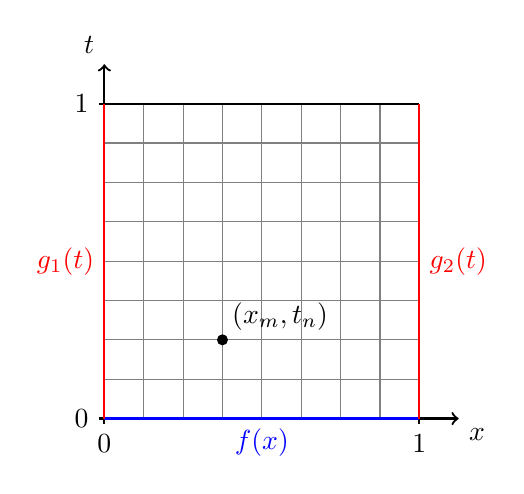
\begin{tikzpicture}
    %grid
    \draw[step=0.5,gray,thin] (0,0) grid (4, 4);

    % axes
    \draw[thick,->] (0,0) -- (4.5,0) node[anchor=north west] {\( x \)};
    \draw[thick,->] (0,0) -- (0,4.5) node[anchor=south east] {\( t \)};

    % lines at y=1 and x=1
    \draw[thick] (-2pt,4) node[anchor=east] {\( 1 \)} -- (4,4) ; 
    \draw[thick] (4,-2pt) node[anchor=north] {\( 1 \)} -- (4,4) ; 
    \draw[thick] (-2pt,0) node[anchor=east] {\( 0 \)} -- (4,0) ; 
    \draw[thick] (0,-2pt) node[anchor=north] {\( 0 \)} -- (0,4) ; 

    % initial condition
    \draw[blue, thick] (0,0) -- node[below] {\( f(x) \)} (4,0); 

    % boundary conditions
    \draw[red, thick] (0,0) -- node[left] {\( g_1(t) \)} (0,4); 
    \draw[red, thick] (4,0)  -- node[right] {\( g_2(t) \)} (4,4); 

    % point in grid
    \fill (1.5, 1) circle (2pt) node[above right] {\( (x_m, t_n) \)};
  \end{tikzpicture}
}
  \caption{The domain \( [0, 1] \times [0, 1] \),
    with boundary and initial conditions
    given by functions \( f, g_1 \) and \( g_2 \).
  }
\end{figure}

A scheme based on forward and backward Euler,
together with a central difference in space, could be:
$$
  \frac{1}{k}\nabla_tU_{m}^{n+1}=\frac{\mu}{h^2}\delta_x^2U_{m}^{n+1}+f(U_{m}^{n} )
$$
which can be rewritten to 
\begin{equation}
  \label{eq:scheme}
  U_{m}^{n+1} = U_{m}^{n} + r (U_{m+1}^{n+1}-2U_{m}^{n+1}+U_{m-1}^{n+1}) + kf(U_{m}^{n}), \quad r = \mu\frac{k}{h^2}
\end{equation}
Time dependent PDEs with diffusion terms should be solved using implicit methods.
This requires solving a nonlinear system for each step.
The following scheme is based on an implicit method
for the diffusion term and an explicit method for the reaction term.
\begin{align}
  \label{eq:scheme_implicit_eq}
    U_{m}^{*} =& U_{m}^{n} +\frac{r}{2}(\delta_x^2 U_{m}^{*} + \delta_x^2 U_{m}^{n} ) + kf(U_{m}^{n}) \\
  \label{eq:scheme_explicit_eq}
    U_{m}^{n+1} =& U_{m}^{*} + \frac{k}{2}(f(U_{m}^{*}) - f(U_{m}^{n}))
\end{align}

\subsection{Stability analysis}

Define the matrix \( S = \text{tridiag}(1, -2, 1) \in \text{Mat}_{M,M}(\mathbb{R}) \).
That is,
\begin{equation}
  \label{eq:Smatrix}
  S = 
  \begin{bmatrix}
    -2 & 1 &  &  & \\
    1& -2 & 1 &  & \\
     & \ddots & \ddots & \ddots & \\
     &  & 1 & -2 & 1\\
     &  &  & 1 & -2\\
  \end{bmatrix},
\end{equation}
and define the vector \( U^n = [U_1^n, U_2^n, \dots, U_M^n]^T \)
by combining the function values at the \( M \) inner points
at a time point \( t_n \) into a vector.

Before we go on with the stability analysis we need some results
concerning the matrix \( S \).

\begin{lemma}
  \label{lemma:S_diagonalizable}
  Let \( S \in \text{Mat}_{M,M}(\mathbb{R}) \) be defined as in \eqref{eq:Smatrix}.
  Then \( S \) is diagonalizable by an orthogonal matrix \( P \).
  That is, \( S = P \Lambda P^T \), for some diagonal matrix \( \Lambda \).
  The eigenvalues of \( S \) are found on the diagonal of \( \Lambda \):
  \[
    \lambda_m = - 4 \sin^2 \phi_m,
  \]
  where \( \phi_m = \frac{m \pi}{2(M+1)} \) for \(m = 1, \dots, M. \)
\end{lemma}
\begin{proof}
    Problem \( 1 \) of exercise set \( 1 \).
\end{proof}

\begin{lemma}
  \label{lemma:existance_of_inverse}
Let \( S \in \text{Mat}_{M,M}(\mathbb{R}) \) be defined as in \eqref{eq:Smatrix},
and let \( r \) be defined as in \eqref{eq:scheme}.
  Then \( \left(I - \frac{r}{2} S\right)\) is invertible.
\end{lemma}
\begin{proof}
  \( I - \frac{r}{2} S \) is invertible iff. all the eigenvalues are nonzero.
  From lemma \ref{lemma:S_diagonalizable} we we have a diagonalization of \( S \). Thus
  \begin{equation*}
      I - \frac{r}{2} S
      = PP^T - \frac{r}{2} P\Lambda P^T
      = P \left(I - \frac{r}{2} \Lambda \right) P^T
  \end{equation*}
  The eigenvalues of \( I - \frac{r}{2}S \) are
  \( 1 - \frac{r}{2} \lambda_m\),
  where the \( \lambda_m \)-s are the eigenvalues of \( S \).
  Observe that \( r > 0 \) and \( \lambda_m < 0 \) for all \( m = 1, \dots, M \).
  Hence
  \[
    1 - \frac{r}{2} \lambda_m > 1 \neq 0,
  \]
  so the matrix is invertible.
\end{proof}

Rewriting \eqref{eq:scheme_implicit_eq} as a matrix-vector equation
and collecting the \( U^* \)-s on the left hand side yields:
\begin{equation}
  \left(I - \frac{r}{2}S\right)U^* = \left(I + kaI + \frac{r}{2}S\right) U^n
\end{equation}

\( I - \frac{r}{2}S \) is invertible
by lemma \ref{lemma:existance_of_inverse}.
We substitute for \( U^* \)
in \eqref{eq:scheme_explicit_eq}
and arrive at an expression for the matrix \( C \)
satisfying \( U^{n+1} = C U^n \).
\begin{align*}
  U^{n+1} &= U^n + \frac{ka}{2}\left(U^*  - U^n\right) \\
          &= \left(1 + \frac{ka}{2}\right) U^* - \frac{ka}{2}U^n \\
          &= \left(1 + \frac{ka}{2}\right) {\left[I - \frac{r}{2}S\right]}^{-1} \left(I + kaI + \frac{r}{2}S\right) U^n - \frac{ka}{2}U^n \\
          &= {\left[I - \frac{r}{2}S\right]}^{-1} \left(\left(1 + \frac{ka}{2}\right)\left(I + kaI + \frac{r}{2}S\right) - \frac{ka}{2}\left(I-\frac{r}{2}S\right)\right) U^n \\
          &= {\left[I - \frac{r}{2}S\right]}^{-1} \left( \left(1+ka+\frac{1}{2}(ka)^2\right)I + \frac{1}{2}\left(1+ka\right)rS\right) U^n
\end{align*}

So
\begin{equation}
    C = {\left[I - \frac{r}{2}S\right]}^{-1} \left( \left(1+ka+\frac{1}{2}(ka)^2\right)I + \frac{1}{2}\left(1+ka\right)rS\right).
  \end{equation}

By exploiting lemma \ref{lemma:S_diagonalizable} we arrive at a diagonalization for \( C \):
\begin{align*}
  C &= {\left[I - \frac{r}{2}S\right]}^{-1} \left( \left(1+ka+\frac{1}{2}(ka)^2\right)I + \frac{1}{2}\left(1+ka\right)rS\right) \\
    &= {\left[PP^T - \frac{r}{2}P\Lambda P^T\right]}^{-1} \left( \left(1+ka+\frac{1}{2}(ka)^2\right)PP^T + \frac{1}{2}\left(1+ka\right)r P\Lambda P^T\right) \\
    &= P{\left[I - \frac{r}{2}\Lambda \right]}^{-1} \left( \left(1+ka+\frac{1}{2}(ka)^2\right)I + \frac{1}{2}\left(1+ka\right)r \Lambda \right) P^T \\
    &= P \Delta P^T
\end{align*}
where
\begin{equation}
    \Delta = {\left[I - \frac{r}{2}\Lambda \right]}^{-1} \left( \left(1+ka+\frac{1}{2}(ka)^2\right)I + \frac{1}{2}\left(1+ka\right)r \Lambda \right)
\end{equation}

We observe that \( C \) is symmetric
since \( C = P \Delta P^T = P \Delta^T P^T = \left(P \Delta P^T\right)^T = C^T \).
This is nice since now the condition \( \rho(C) \le 1 + \nu k \) is
both \textit{necessary} and sufficient for stability
when we use \( ||\cdot||_{2,h} \).
In particular, for a symmetric matrix \( C \),
we have that \( ||C||_{2,h} = \rho(C) \).

The eigenvalues for \( C \) are found on the diagonal of \( \Delta \):
\begin{equation}
  \Delta_m =
      \frac{\left(1+ka+\frac{1}{2}(ka)^2\right) + \frac{1}{2}\left(1+ka\right)r \lambda_m}
      {1 - \frac{r}{2} \lambda_m}
\end{equation}

Bounding \( \rho(C) = \max_{m} \lvert \Delta_m \rvert \):
\begin{align*}
  \left\lvert \Delta_m \right\rvert &= 
\left\lvert \frac{\left(1+ka+\frac{1}{2}(ka)^2\right) + \frac{1}{2}\left(1+ka\right)r \lambda_m}
{1 - \frac{r}{2} \lambda_m} \right\rvert \\
 &= 
 \left\lvert \left(1+ka\right)\frac{1+\frac{1}{2}r \lambda_m}{1 - \frac{1}{2}r \lambda_m} + \frac{1}{2}(ka)^2 \frac{1}{1 - \frac{1}{2}r \lambda_m} \right\rvert \\
 &\le \left\lvert \left(1+ka\right) \right\rvert \left\lvert \frac{1+\frac{1}{2}r \lambda_m}{1 - \frac{1}{2}r \lambda_m} \right\rvert + \frac{1}{2}(ka)^2 \left\lvert\frac{1}{1 - \frac{1}{2}r \lambda_m} \right\rvert \\
 \intertext{
   Note that \( -1 < \lambda_m < 0  \) for all \( m = 1, \dots, M \).
   In addition, the step size \( k \) is bounded by some constant
   \( T \) (having a step size larger than the length of the time domain
   do not make sence).
  We simplify further:
}
 \left\lvert \Delta_m \right\rvert
 &\le \left\lvert 1 + ka \right\rvert + \frac{1}{2} (ka)^2 \\
 &= 1 + (\lvert a \rvert + \frac{1}{2}k a^2 )k \\
 &\le 1 + (\lvert a \rvert + \frac{1}{2}T a^2)k \\
 &= 1 + \nu k
\end{align*}

Finally, we have arrived at the expression needed for stability
without imposing any conditions on the scheme.
We summarize our discussion in a theorem.

\begin{theorem}
    \label{stability}
  The scheme given in equations \eqref{eq:scheme_implicit_eq}
  and \eqref{eq:scheme_explicit_eq} is unconditionally stable.
\end{theorem}

\subsection{Consistency}
We also wish to show that the method is consistent. 
\begin{lemma}
    \label{central_difference}
    $$\delta_x^2u_{m}^{n} = h^2\partial_x^2 u_{m}^{n} + \mathcal{O}(h^4)$$
\end{lemma}
\begin{proof}
    $$\delta_x^2u_{m}^{n} = u_{m+1}^{n} - 2 u_{m}^{n} + u_{m-1}^{n}$$
    Then Taylor expand around $u_{m}^{n}$.
    \begin{align*}
        \delta_x^2u_{m}^{n} =& u_{m}^{n}  + h\partial_xu_{m}^{n} + \frac{h^2}{2}\partial_x^2 + \frac{h^3}{3!}\partial_x^3 u_{m}^{n} + \frac{h^4}{4!}\partial_x^4 u_{m}^{n} + \mathcal{O}(h^5) \\
        -&2u_{m}^{n} \\
        +& u_{m}^{n} - h\partial_xu_{m}^{n} + \frac{h^2}{2}\partial_x^2 u_{m}^{n} - \frac{h^3}{3!}\partial_x^3u_{m}^{n} + \frac{h^4}{4!}\partial_x^4 u_{m}^{n} + \mathcal{O}(h^5) \\
        =& h^2\partial_x^2 u_{m}^{n} + \frac{h^4}{12}\partial_x^4 u_{m}^{n} + \mathcal{O}(h^5) \\
        =&  h^2\partial_x^2 u_{m}^{n} + \mathcal{O}(h^4)
    \end{align*}
\end{proof}

\begin{theorem}
    \label{consistent}
    Given that $u$ is sufficiently smooth,  $f$ is of the form $f(u)=au, a\in \mathbb{R}$ and $k \neq \frac{-2}{a}$, the local truncation error of the method is of order $k^2 + h^2.$
\end{theorem}

\begin{proof}
    For the boundaries, $\tau_0=\tau_{M+1}= 0$, since we have Dirichlet boundary conditions and the approximation is exact.
    For the inner points we rewrite (\ref{eq:scheme_explicit_eq}) to be an explicit equation for $U_m^*$
    $$ U_{m}^{*}= \frac{U_{m}^{n+1}+\frac{ka}{2}U_{m}^{n}}{1+\frac{ka}{2}}.$$
    This is then substituted into (\ref{eq:scheme_implicit_eq}) to remove $U_{m}^{*}$ from the equation
    $$\frac{U_{m}^{n+1}+\frac{ka}{2}U_{m}^{n}}{1+\frac{ka}{2}} = (1+ka)U_{m}^{n}+\frac{r}{2}\left( \frac{\delta_x^2(U_{m}^{n+1}+\frac{ka}{2}U_{m}^{n})}{1+\frac{ka}{2}}  + \delta_x^2 U_{m}^{n}\right).$$
    We then multiply by $(1+\frac{ka}{2})$ and rearrange the terms to
    $$ U_{m}^{n+1}=(1+ ka + \frac{k^2a^2}{2})U_{m}^{n} + \frac{r}{2}\left((1+ka)\delta_x^2U_{m}^{n} +\delta_x^2U_{m}^{n+1}\right).$$
    Then the approximations are replaced by $u$ and the local truncation error is therefore introduced
    $$ k\tau_m^n + u_{m}^{n+1} = (1+ ka + \frac{k^2a^2}{2})u_{m}^{n} + \frac{r}{2}\left((1+ka)\delta_x^2u_{m}^{n} +\delta_x^2u_{m}^{n+1}\right).$$
    We then use lemma \ref{central_difference} for the central differences and Taylor expand around $u_{m}^{n}$
    \begin{align*}
        k \tau_m^n =& \left( 1 + ka +\frac{k^2a^2}{2}\right)u_{m}^{n} - u_{m}^{n+1}+\frac{\mu k}{2h^2} \left(h^2\partial_x^2 u_{m}^{n+1} + \left( 1+ka \right) h^2 \partial_x^2u_{m}^{n} + \mathcal{O}(h^4)\right) \\
        k \tau_m^n =& \left( 1 + ka + \frac{k^2a^2}{2}\right)u_{m}^{n} - u_{m}^{n} - k \partial_tu_{m}^{n} - \frac{k^2}{2} \partial_t^2 u_{m}^{n} + \mathcal{O}(k^3)  \\
        +& \frac{\mu k}{2}\left( \partial_x^2 \left( u_{m}^{n} + k \partial_t u_{m}^{n} + \mathcal{O}(k^2)\right) + \left( 1 + ka\right) \partial_x^2  u_{m}^{n} \right) + \mathcal{O}(kh^2).
    \end{align*}
    This expression is then divided by $k$ and rearranged to 
    $$\tau_m^n = a u_{m}^{n} - \partial_tu_{m}^{n} + 2 \frac{\mu}{2}\left( \partial_x^2 u_{m}^{n}\right) +  \frac{ka^2}{2}u_{m}^{n}  - \frac{k}{2} \partial_t^2 u_{m}^{n} + \frac{\mu }{2}\left( k \partial_x^2 \partial_t u_{m}^{n}  + ka \partial_x^2  u_{m}^{n} \right) + \mathcal{O}(h^2 + k^2).$$
    The first three terms are simply (\ref{eq:original_eq}) with all terms moved to the right hand side. Some terms can also be rewritten using (\ref{eq:original_eq}), $\mu \partial_x^2u_{m}^{n} = \partial_t u_{m}^{n} - au_{m}^{n}$, yielding
    \begin{align*}
        \tau_m^n = \frac{ka^2}{2}u_{m}^{n}  - \frac{k}{2} \partial_t^2 u_{m}^{n} +& \frac{k}{2} \partial_t \left(\partial_t u_{m}^{n}   - au_{m}^{n} \right) + \frac{ka}{2} \left( \partial_t  u_{m}^{n} - a u_{m}^{n}\right)+ \mathcal{O}(h^2 + k^2) \\
        \tau_m^n = \frac{ka^2}{2}u_{m}^{n} - \frac{ka^2}{2}u_{m}^{n}  -& \frac{k}{2} \partial_t^2 u_{m}^{n} + \frac{k}{2} \partial_t^2 u_{m}^{n} - \frac{ka}{2} \partial_t u_{m}^{n} + \frac{ka}{2} \partial_t  u_{m}^{n}+ \mathcal{O}(h^2 + k^2) \\
        \tau_m^n =& \mathcal{O}(h^2 + k^2) \\
    \end{align*}
\end{proof}

\begin{corollary}
    \label{corollary:norm_tau}
    $\lVert\tau^s \lVert_{2, h} =\mathcal{O}(h^2+k^2)$
\end{corollary}

\begin{proof}
We use the definition of $\lVert\cdot\lVert_{2,h}$ and theorem \ref{consistent} for an upper bound of $\lvert \tau_m^n\lvert$
    $$\lVert\tau^s \lVert_{2, h} = \sqrt{h}\left( \sum_{i=0}^{M+1} \lvert\tau^s_i \lvert^2 \right)^\frac{1}{2} \leq \sqrt{h}\left( \sum_{i=0}^{M+1} A(k^2+h^2) \right)^\frac{1}{2} = \sqrt{h}\left[ (M+1) A^2(k^2+k^2)^2 \right]^\frac{1}{2}$$
    and using that $h = \frac{1}{M+1}$
    $$\lVert\tau^s \lVert_{2, h} = \frac{\sqrt{h}}{\sqrt{h}}A(k^2+h^2) = A(k^2+h^2).$$
\end{proof}
\begin{theorem}
    \label{convergence_lax}
    Given that $u$ is sufficiently smooth,  $f$ is of the form $f(u)=au, a\in \mathbb{R}$ and $k \neq \frac{-2}{a}$, the method is convergent.
\end{theorem}

\begin{proof}
    The method is stable, (\ref{stability}), and consistent, (\ref{consistent}), and therefore convergent by Lax' equivalence theorem.
\end{proof}


\begin{theorem}
  \label{thm:conv_order}
    The method is convergent of order $h^2+k^2$ with respect to $\lVert\cdot \lVert_{2, h}$.
\end{theorem}

\begin{proof}
    The scheme can be written in the form
    $$\left(I - \frac{r}{2}S \right)U_{m}^{n+1} = \left( \left(1+ka+\frac{1}{2}(ka)^2\right)I + \frac{1}{2}\left(1+ka\right)rS\right)U_{m}^n$$
    or using $A = \left(I - \frac{r}{2}S \right)$ and $B = \left( \left(1+ka+\frac{1}{2}(ka)^2\right)I + \frac{1}{2}\left(1+ka\right)rS\right)$ as
    $$AU_{m}^{n+1} = BU_{m}^{n+1}.$$
    If we place $U_m^n - u_m^n$ into the equation instead, we get
    $$AE^{n+1} = BE^n - k\tau^n$$
    exchanging $n+1$ with $n$, multiplying by $A^{-1}$, which exists given lemma \ref{lemma:existance_of_inverse}
    $$E^n = A^{-1}BE^{n-1} -kA^{-1}\tau^n$$
    we set $q^{n-1}= -kA^{-1}\tau^n$ and $C=A^{-1}B$
    $$E^n = CE^{n-1}+q^{n-1}$$
    and by using the term recursively, we get
    $$E^n = C^nE^{0}+C^{n-1}q^0 + C^{n-2}q^1 + \dots + C q^{n-2} +  q^{n-1}.$$
    Taking the norm on both sides and using stability from theorem \ref{stability} to give a bound $L$ for $\lVert C^n \lVert$
    $$\lVert E^n\lVert  \leq L\sum_{s=0}^{n-1}\lVert q^s \lVert$$
    we the use that 
    $$\lVert q^s \lVert \leq k \lVert A^{-1} \lVert \lVert\tau^s \lVert \leq k \tilde{K} \lVert\tau^s \lVert$$
    and, using $nk\leq Nk=T$, obtain
    $$\lVert E^n \lVert \leq L \tilde{K}nk \max_{0\leq s \leq n-1} \lVert \tau^s\lVert \leq L \tilde{K}T\max_{0\leq s \leq n-1} \lVert \tau^s\lVert.$$
    Using $\lVert \cdot \lVert_{2, h}$ as the norm we get by corollary \ref{corollary:norm_tau}
    $$\lVert E^n \lVert_{2, h} \leq L \tilde{K}TA(k^2+h^2)$$
\end{proof}

\subsection{Numerical experiments}
We use the following solution to construct a test equation:
\begin{equation}
  \tilde{u}(t, x) = \text{e}^{-(\mu b + a)t} \sin (bx + \varphi)
\end{equation}
where \( \mu  \) and \( a \) are the constants from the original problem
(\eqref{eq:original_eq}).
Then we set \( \mu = 1/5, b = 3\pi/2, a = 1 \) and \( \varphi = \pi/4 \).
The convergence plots (\ref{fig:conv_plot})
align with the results from the theory section (\ref{thm:conv_order}).
\begin{figure}[!h]
    \centering
    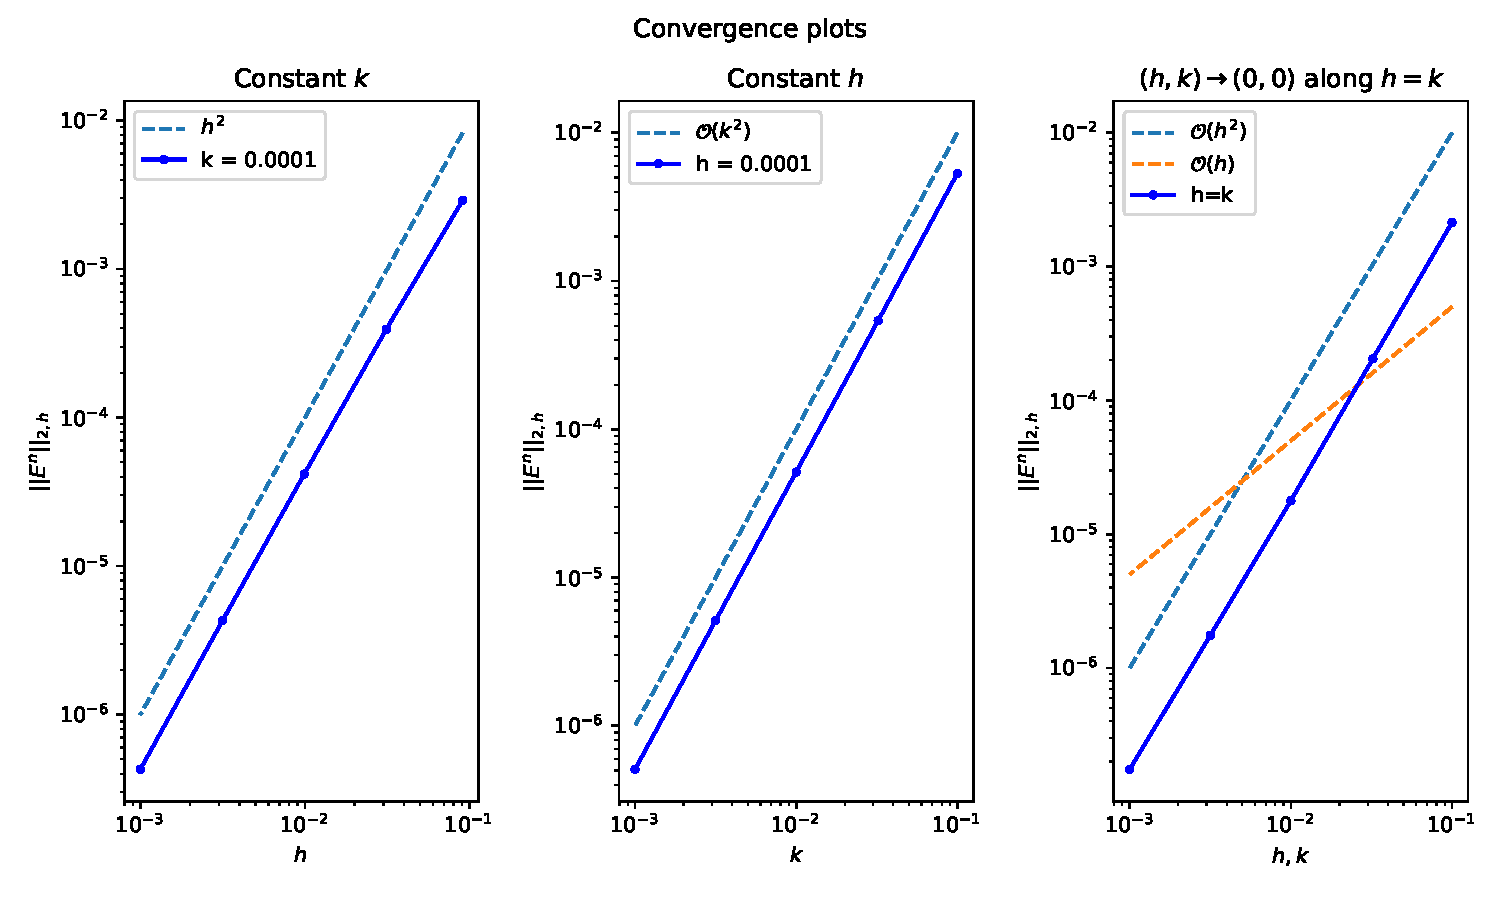
\includegraphics[width=\textwidth]{Images/plots/task1_error.pdf}
    \caption{As long as one of the step sizes (either \( k\) or \( h \)
      is kept small enough, we get quadratic convergence.
      Since we are solving the equation on the grid 
      \( [0,1] \times [0,1] \) it is reasonable to let
      \( h=k \to 0 \).
    }
    \label{fig:conv_plot}
\end{figure}
